%!TEX root = ../dokumentation.tex

% Kapitel über Schaltungen, Signalerzeugung und -verarbeitung
\chapter{Schaltungen}


% Section über Sender-Schaltung, Signalerzeugung
\section{Sender}
Der Ultraschallsender wird durch ein $40 kHz$-Signal angeregt und erzeugt einen Schallkegel mit etwa $80^\circ$ Abstrahlwinkel. Der Schallpegel sollte dabei möglichst hoch sein, um die erfolgreiche Signalauswertung des reflektierten Signals auch über weite Distanzen und geringen Reflexionsfaktoren zu ermöglichen. Der hohe Abstrahlwinkel hat auch zur Folge, dass nur ein Bruchteil der Schallwelle am Objekt auftrifft und reflektiert werden kann. Es wird empfohlen, den Sender mit einem Rechtecksignal anzusteuern. Durch sein schmales Frequenzband schwingt er dennoch Sinus-förmig und nimmt dabei am meisten Energie auf. Der Sender besteht aus einem Piezoelement, dessen vereinfachtes Ersatzschaltbild ein Kondensator ist. Laut Datenblatt besitzt er eine Kapazität von $2.55nF$.


\subsection{Signalerzeugung}
Das Rechtecksignal wird von dem Mikrocontroller erzeugt. Er besitzt einen Hardwarezähler, der mit einem Ausgangspin verbunden werden kann. Damit lässt sich ein präzises Signal erzeugen, ohne die Rechenleistung des Controllers einzuschränken.\\
Der Sender hat eine maximale Spitze-Spitze-Spannung von $U_{SS} = 20V$, das ausgegebene Signal des Mikrocontrollers wechselt jedoch nur zwischen $0V$ und $5V$. Die Sendeleistung wäre zu schwach, außerdem sollte der Ausgang des Mikrocontrollers nicht direkt belastet werden, da er nur sehr begrenzt Strom liefern kann. Aus diesen Gründen wurden mehrere Sendeverstärker entwickelt und untersucht, ob sie geeignet sind.



\subsection{Erste Schaltung: Verstärkung mit Operationsverstärker}
\subsubsection{Idee} % FIXME Differenzverstärker
Mithilfe eines Operationsverstärkers lassen sich einfach Spannungen verstärken. Mit einer Komparatorschaltung kann das $0/5V$-Signal auf $-10/+10V$ umgesetzt werden. Der Operationsverstärker \textit{LM258} ist zum Einsatz gekommen, da seine Spannungsversorgung sehr hoch und flexibel gewählt werden kann und er eine relativ hohe Bandweite von $1.1MHz$ aufweist.
\begin{figure}[H]
\centering
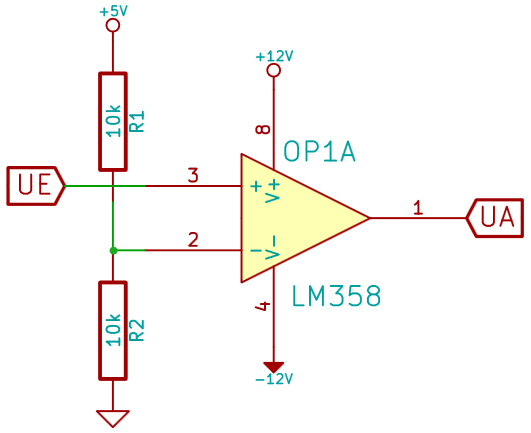
\includegraphics[scale=0.5]{images/komparatorschaltung.jpg}
\caption{Einfache Komparatorschaltung zum Umsetzen der Spannungen} \label{img:I1}
\end{figure}

\subsubsection{Problematik}
Bereits bei der Planung der Schaltung wurde befürchtet, dass der maximale Strom des Operationsverstärkers für ein scharfes Signal sehr knapp dimensioniert ist ($I_{Source}=30mA; I_{Sink}=40mA$). Nimmt man an, der Operationsverstärker besitzt einen Ausgangswiderstand von $0 \Omega$ und die Ladespannung beträgt $20V$, ist die Zeit zum vollständigen Laden des Senders:
\begin{equation}
t=\frac{Q}{I}=\frac{C*U}{I}=\frac{2.55nF*20V}{30mA}=1.7\mu s
\end{equation}
Im Vergleich zur Pulsdauer von $12.5\mu s$ ist dieser Wert in Ordnung. Allerdings besitzt nur ein idealer Operationsverstärker einen $0\Omega$-Ausgangswiderstand und der Sender ist auch kein idealer Kondensator ohne seriellen Widerstand. Deshalb wurde erwartet, dass die Flanken etwas abgeflacht werden.\\
Tatsächlich wurde jedoch ein viel wichtigerer Wert im Datenblatt übersehen. Die \textit{Slew Rate} gibt an, wie schnell sich die Spannung des OPs ändern kann. Beim \textit{LM258} beträgt sie $0.6V/\mu s$. Das Ausgangssignal entsprach aus diesem Grund einem Dreiecksignal und schwankte nur um wenige Volt.
% Bild von Simulation
\begin{figure}[H] %TODO: Kontrast von Bild erhöhen. Außerdem stimmen die 20V/µs nur ungefähr.
\centering
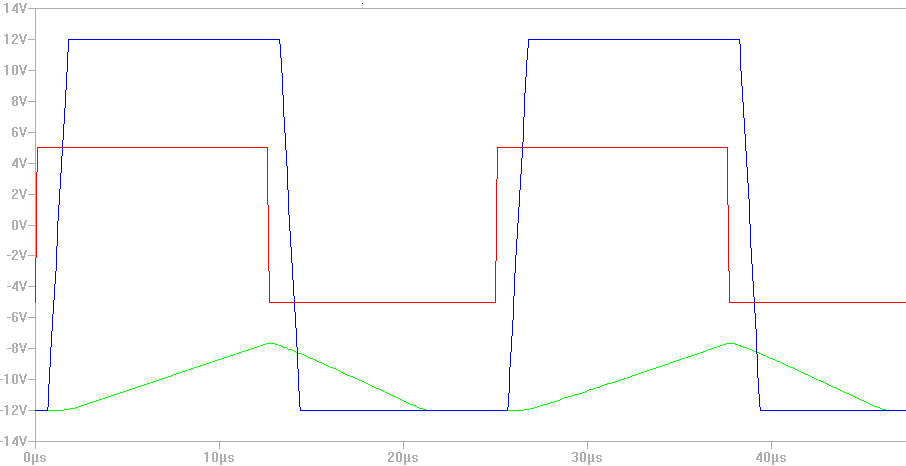
\includegraphics[scale=0.6]{images/signalverlauf_opamps.png}
\caption{Simulierter Signalverlauf von zwei Operationsverstärkern. Rot: Ansteuersignal. Grün: Slew-Rate $0.6V/\mu s$. Blau: Slew-Rate $20V/\mu s$.} \label{img:I2}
\end{figure}

\subsubsection{Fazit}
Die Spannungsverstärkung mit dem Operationsverstärker \textit{LM258} hat sich als nicht praktikabel herausgestellt, da er zu langsam reagiert. Für diese Zwecke können jedoch spezielle \textit{Komparatoren} verwendet werden, die sich wie Operationsverstärker verhalten, nur viel schneller und ungenauer sind. Die Genauigkeit spielt beim Umschalten keine Rolle.\\
Nach dieser Feststellung wurden Schaltungen mit Transistoren untersucht, da sie höhere Leistungen und schnellere Reaktionszeiten zulassen.


\subsection{Zweite Schaltung: Verstärkung mit Transistor}
%TODO Sollen Berechnungen von Strömen und Widerständen hier noch rein?
Der Bipolartransistor ist ein stromgesteuertes Halbleiterbauelement, der als Verstärker und Schalter eingesetzt wird. Die Emitterschaltung eignet sich für hohe Spannungs- und Stromverstärkungen. Im übersteuerten Zustand lassen sich damit ohmsche Lasten elektronisch schalten. Gemeinsamer Bezugspunkt ist der Emitter - daher der Name der Schaltung. Der Strom von Basis zu Emitter steuert den maximalen Stromfluss der Schaltstrecke von Kollektor zu Emitter. Um ein digitales Signal zu verstärken, wird es über den Basiswiderstand auf den Transistor gegeben und ein weiterer Widerstand vor den Kollektor zur resultierenden Spannung geschaltet. Leitet der Transistor, fällt die Spannung am Widerstand ab. Sperrt er, fällt an ihm die Spannung ab und der Widerstand zieht das Potential vor dem Transistor auf den gewünschten Wert. Das resultierende Signal ist um $180^\circ$ phasenverdreht, d.h. es wird invertiert aber nicht verzögert. Der Transistor wird im übersteuerten Bereich betrieben, damit er sauber durchschalten kann und keine Verluste durch Spannungsabfall an ihm entstehen. \\


\subsubsection{Spannungsbereich ausschöpfen}
Als Spannungsversorgung stehen $+5V$, $+12V$ und $-12V$ zur Verfügung. Es gibt verschiedene Schaltungen, die unterschiedliche Spannungsbereiche bieten:
\begin{description}
	\item[NPN-Transistor:] Gebräuchliche Schaltung um einen Schalter mit einen Transistor zu realisieren. Die $5V$ werden auf $12V$ verstärkt.
	\item[PNP-Transistor:] Mit nur einem Transistor kann das Signal auf $-12V$-$+5V$ umgesetzt werden. Die Spitze-Spitze-Spannung beträgt $17V$.
	\item[Zwei Transistoren:] Kombiniert man beide Verstärker, kann das Signal auf $-12V$-$+12V$ verstärkt werden. Da die Spitze-Spitze-Spannung des Senders um $4V$ überstiegen wird, muss sie mit einer Z-Diode begrenzt werden. Sie wird in Reihe entgegen der Spannung geschaltet, sodass an ihr die nötige Spannung abfällt.
	\item[Wechselsignal:] Der Sender ist nicht gegen Masse geschaltet, sondern erhält am anderen Pin das invertierte Signal. Dadurch lässt sich die Spitze-Spitze-Spannung verdoppeln. Es wird mindestens ein weiterer Transistor benötigt, um die zweite Seite zu beschalten. Dafür kann das Ausgangssignal des ersten Transistors genutzt werden, da es um $180^\circ$ phasenverdreht zum Eingangssignal ist. Der Vorteil dieser Schaltung ist, dass die Spannung halbiert werden kann, ohne Sendeleistung einzubüßen.
\end{description}

\begin{figure}[H]
\centering
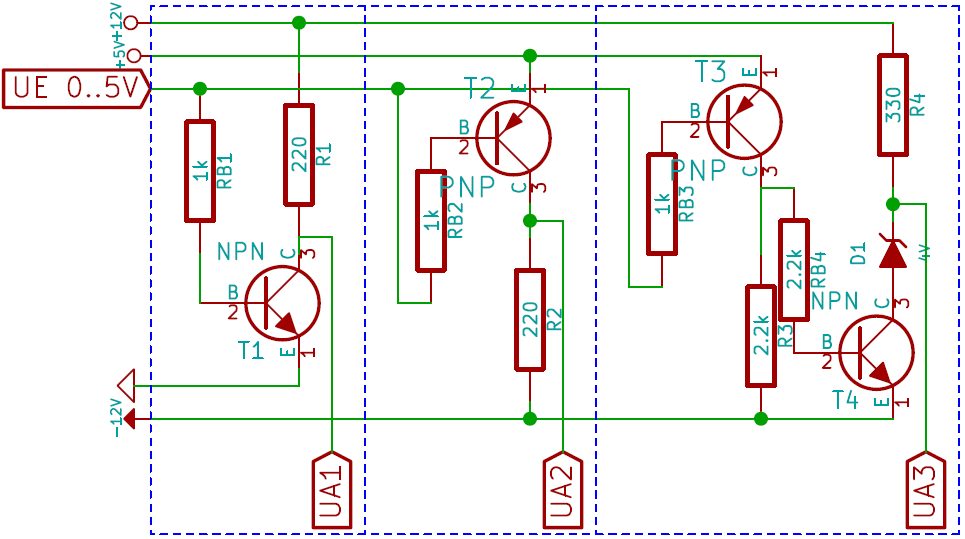
\includegraphics[scale=0.6]{images/transistorschaltungen.png}
\caption{Verstärkungsschaltungen für $12V$, $17V$ und $20V$pannung} \label{img:I3}
\end{figure}

\subsubsection{Nachteile}
Die Emitterschaltung ist eine einfache Verstärkerschaltung und eignet sich hervorragend um ohmsche Lasten zu schalten. Der Sender ist jedoch eine kapazitive Last, die zu jeder Flanke geladen oder entladen werden muss. Über den Lastwiderstand wird die Kapazität geladen, wenn der Transistor sperrt. Solange er leitend ist, fließt ein konstanter Strom über diesen Widerstand, der für den Sender nicht benötigt wird. Die Dimensionierung der Lastwiderstände ist deshalb ein Kompromiss aus unnötigen Stromfluss vermeiden und eine gewisse Flankensteilheit durch die RC-Ladekurve zu erreichen. Statt einem Ein- und Ausschalten wäre ein Umschalten zwischen zwei Spannungen sinnvoller. Diesen Ansatz verfolgt die nächste entworfene Schaltung.

%TODO Bild überarbeiten
\begin{figure}[H]
\centering
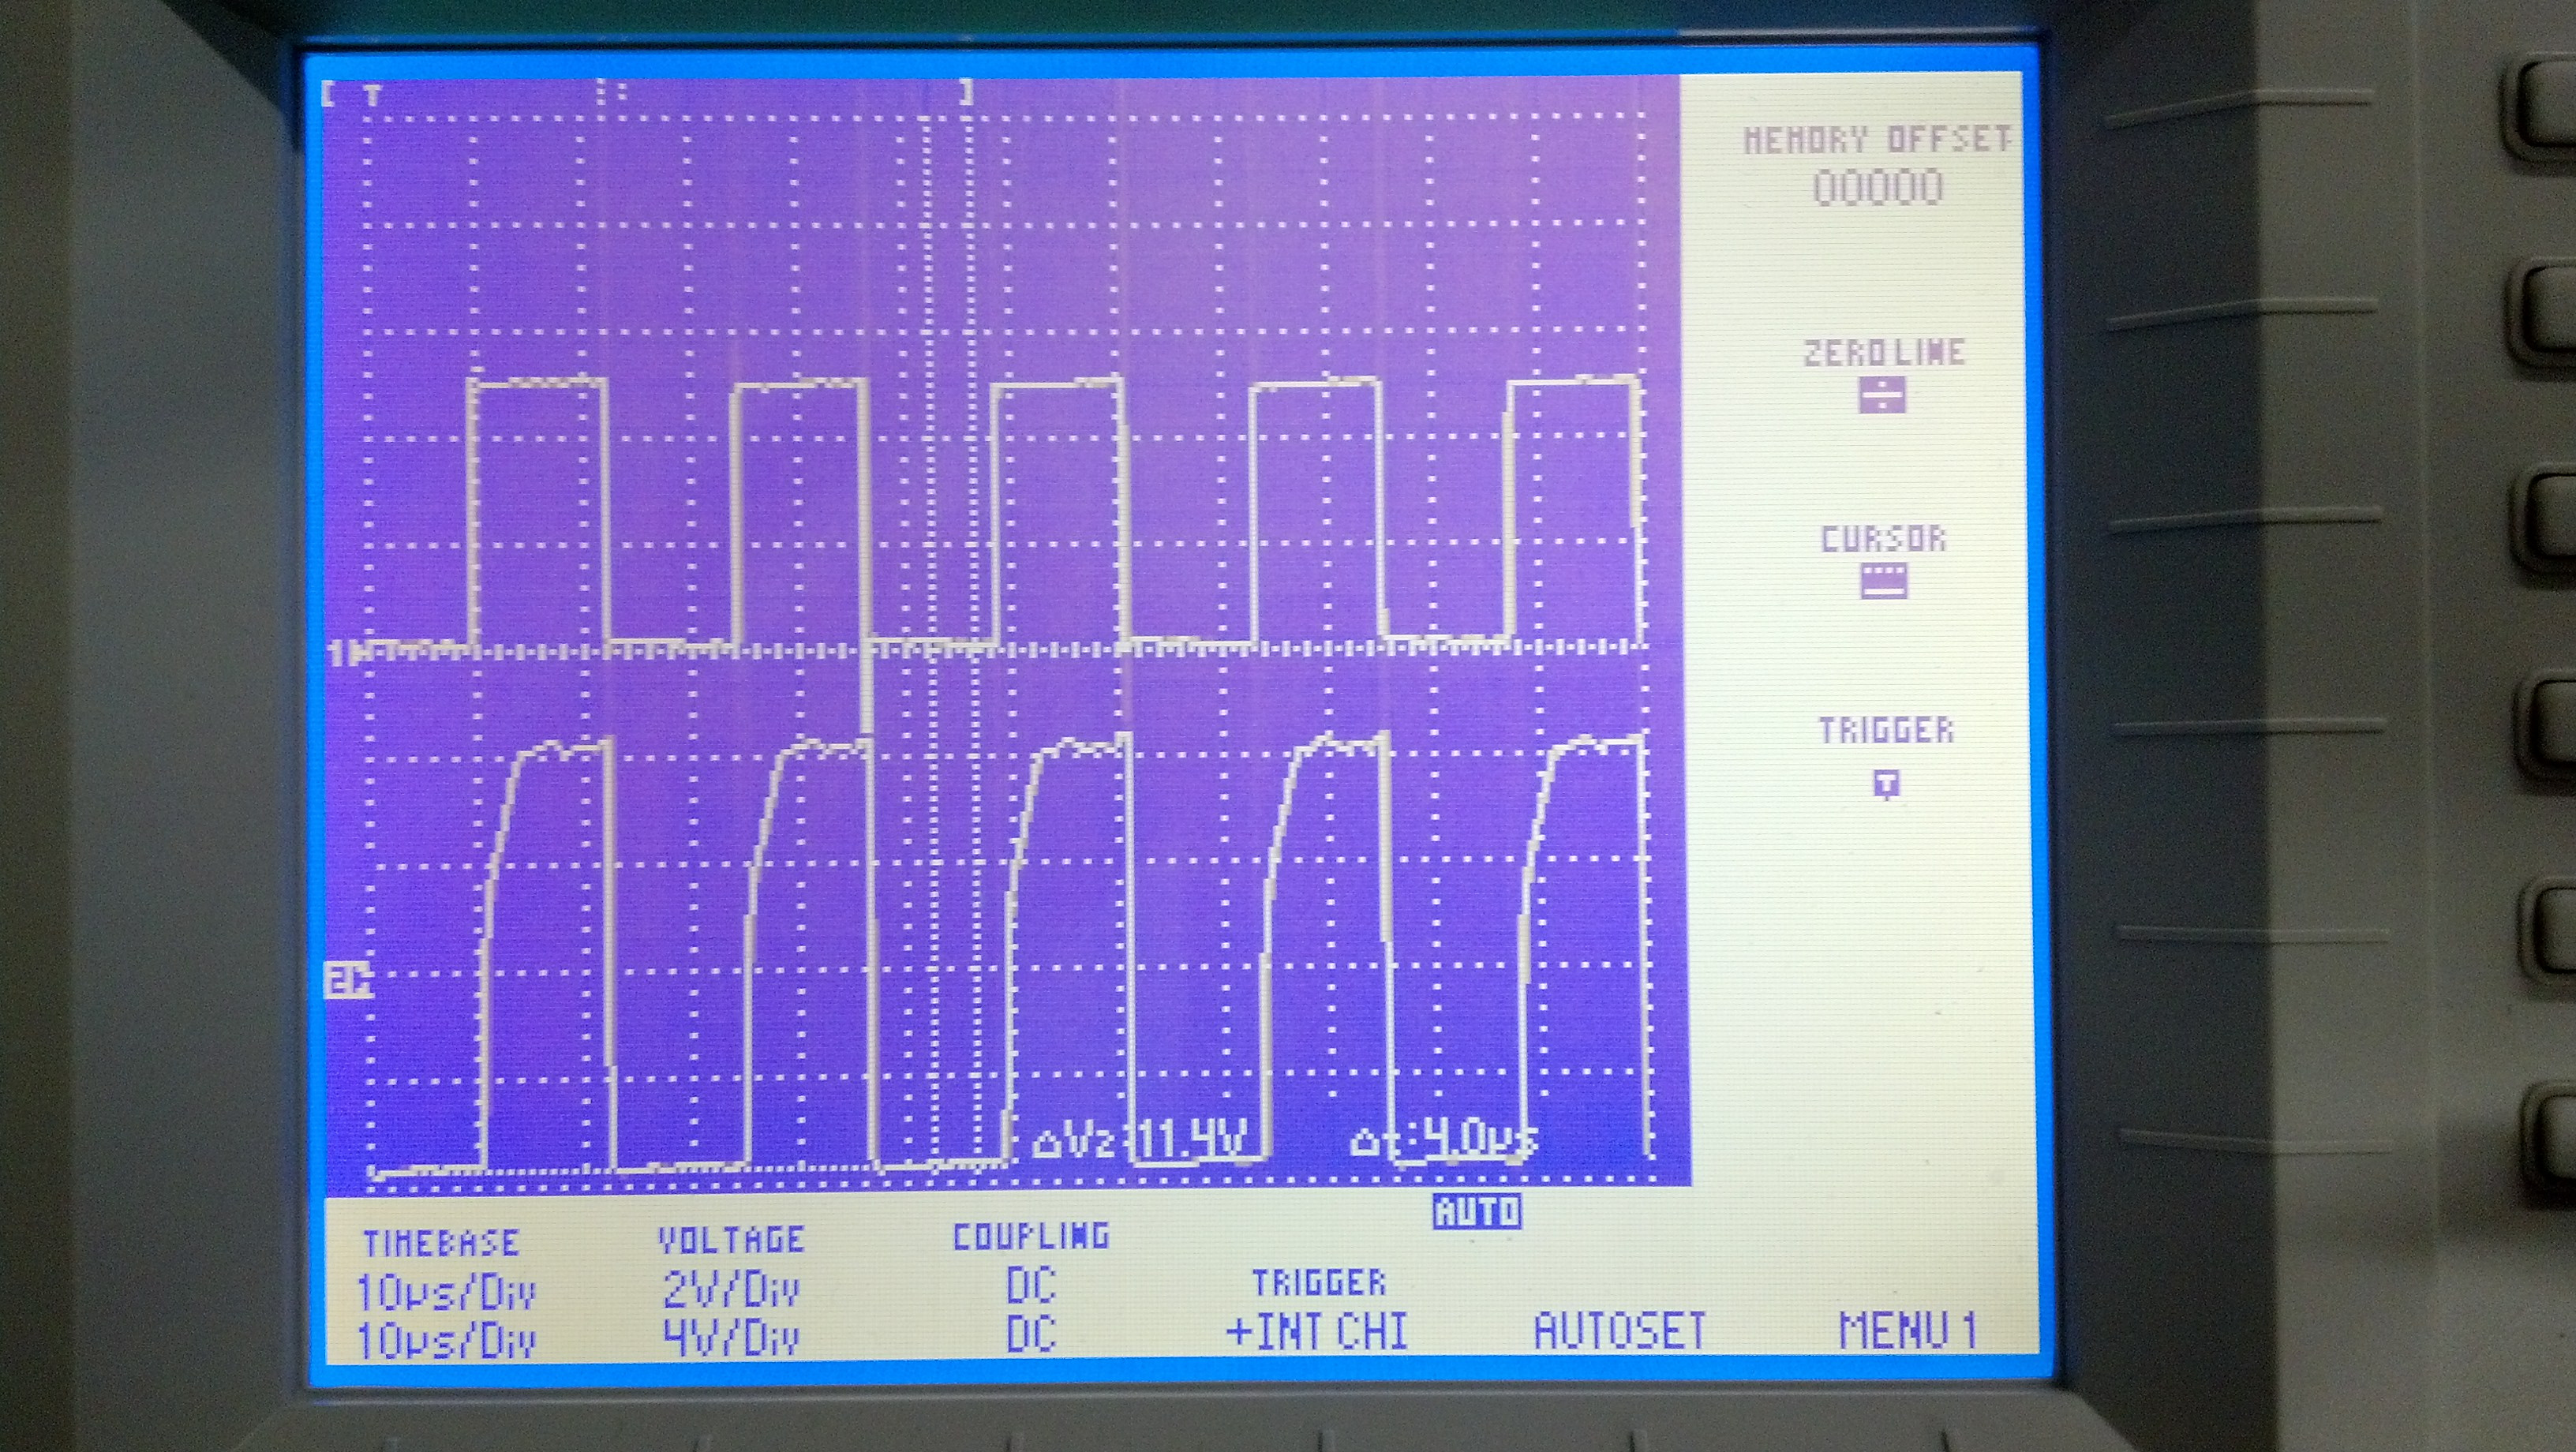
\includegraphics[scale=0.14]{oszi/15-04-01/2.jpg}
\caption{Ladekurven an einer Kapazität} \label{img:I4}
\end{figure}

\subsection{Dritte Schaltung: Gegentaktstufe}
Anstatt die Spannung über den Lastwiderstand am Kollektor eines Transistors auf den richtigen Wert zu ziehen, kann die Spannung über zwei Transistoren, die sich im Gegentakt öffnen und schließen, direkt erreicht werden. Die Vorteile dabei sind, dass der Sender über sehr kleine Widerstände schnell geladen werden kann und dennoch kein unnötiger Stromfluss entsteht. Das Prinzip der Gegentaktstufe wird in verschiedenen Bereichen angewendet: Von schnellen Logik-ICs über verschiedene Treiberbausteine bis hin zu Leistungsendstufen. Durch die Symmetrie und den geringen Eigenstromverbrauch lassen sich hohe Lasten sehr schnell An- und Abschalten. Allerdings ist eine Gegentaktstufe nicht linear, wodurch sie meist ungeeignet für analoge Anwendungen ist.



\subsubsection{Gleichzeitiges Öffnen der Transistoren}
Ein hohes Risiko der Schaltung ist, dass ein Kurzschluss entsteht, sobald beide Transistoren gleichzeitig geöffnet sind. Die hohen Ströme würden nicht zuletzt den thermischen Tod der Transistoren bedeuten. Die Schaltung muss so gestaltet werden, dass ein gleichzeitiges Öffnen nicht möglich ist. Durch folgenden Aufbau kann das erreicht werden:\\
Die Emitter beider Transistoren werden zusammengelegt. An dieser Stelle wird auch der Sender angeschlossen. Ein NPN-Transistor öffnet nur, wenn ein Strom von Basis zu Emitter fließt. Für den PNP-Transistor muss er in die andere Richtung fließen. Werden nun auch die Basispins dieser beiden Transistoren verbunden, kann nur einer der zwei Fälle auftreten - ein gleichzeitiges Öffnen ist deshalb nicht mehr möglich.
%TODO Nummern ins Bild und im Text verlinken
\begin{figure}[H]
\centering
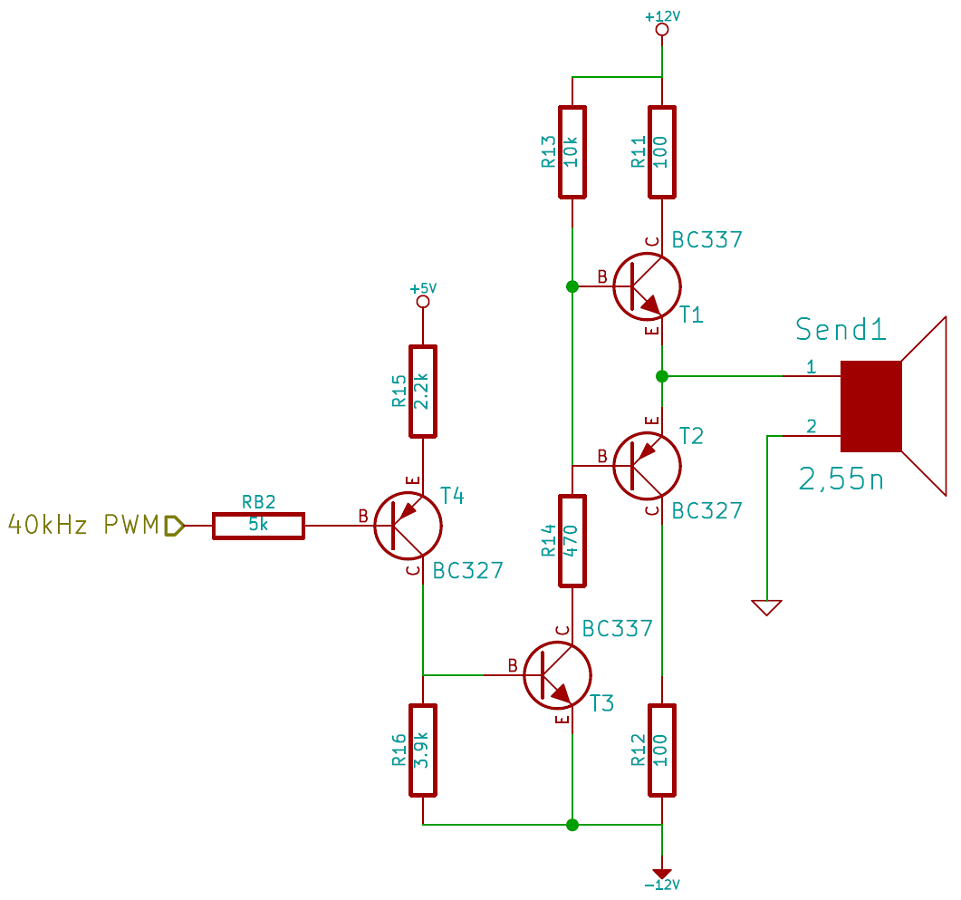
\includegraphics[scale=0.6]{images/push_pull.png}
\caption{Gegentaktstufe als Verstärkerschaltungen} \label{img:I5}
\end{figure}


\subsubsection{Verzögertes Schließen, langsame Reaktionen}
Dioden haben an den Übergängen der Dotierungen kapazitive Eigenschaften. Besonders bei hohen Spannungen wirken sie sich sehr negativ auf die Schaltgeschwindigkeit aus, da die Ladung erst abtransportiert werden muss, bevor sich der Zustand des Transistors ändert. Das führt dazu, dass sie zu spät schließen und die Signale verformt werden. Über mehrere Transistoren summiert sich dieser Effekt auf. Anfangs wurde versucht, die Steuerspannung mithilfe von in Reihe geschalteten Zener-Dioden zu begrenzen. Auch eine Diode von Basis zu Kollektor (NPN), bzw von Kollektor zur Basis (PNP) verringert die Schaltgeschwindigkeit. Überschüssige Ladungsträger fließen über die niederohmige Kollektor-Emitter-Strecke ab, wodurch ein Übersättigen des Transistors vermieden wird. Bei der Gegentaktstufe tritt jedoch der Fall ein, indem der Sender vollständig geladen ist und kein Strom mehr fließt. Ohne Stromfluss fällt an den Z-Dioden keine Spannung ab und die Transistoren übersättigen erneut.\\ %TODO Warum schlechtes Wort?!
Eine akzeptable Lösung wurde gefunden, indem die Arbeitspunkte der Transistoren über Widerstandsverhältnisse (R13 und R14) angepasst wurden. Mithilfe von Schaltungssimulationen konnten die Verhältnisse genau bestimmt werden, bei denen die Transistoren noch sauber schalten und gleichzeitig vor dem Schließen kaum Ladungsträger abtransportiert werden müssen. Die Simulationen waren so genau, dass mit nur geringfügigen Änderungen der Widerstandswerte auch in der Realität optimale Ergebnisse erzielt wurden.

\subsubsection{Aufbau und Funktionsweise}
Drei Stufen


\subsubsection{Fazit}


\subsection{Oberwellen - der Kampf gegen Windmühlen}




% Section über Empfänger und Signalauswertung
\section{Empfänger}
Der Empfänger ist einer der wichtigsten Bausteine bei der Abstandsmessung mit Ultraschall. Nur durch eine zuverlässige Signalverarbeitung kann der Zeitpunkt exakt bestimmt werden, an dem das Signal eingetroffen ist. Im Prinzip gibt es zwei Möglichkeiten die Signalauswertung durchzuführen:
\begin{description} % FIXME: Vielleicht in eigenen sections sinnvoll
	\item[Signalauswertung mit AD-Wandler:] Das empfangene Signal wird vorverstärkt und ständig von einem AD-Wandler ausgelesen. Die Auswertung kann über einfache Schwellwerte bis hin zu komplexen Filterfunktionen, z.B. mithilfe einer Fourier-Transformation, beliebig aufwendig gestaltet werden. Eine Signalvorverarbeitung ist auch denkbar, z.B. Gleichrichten und Glätten, wenn nur die Auslenkung betrachtet wird. Software kann sich auf die Umgebungsbedingungen anpassen, ist jedoch ungenauer und langsamer als die entsprechende Hardwarelösung. Eine genaue Frequenzauswertung erfordert eine hohe Abtastrate und komplexe Software, die dementsprechend auch Rechenleistung benötigt.
	\item[Schwellwertschalter auf einem Interrupt-Eingang:] Hardware übernimmt die Signalverarbeitung mit Verstärkern und Frequenzfiltern. Anschließend schalten die Signalspitzen einen Transistor, der als Schwellwertschalter dient. Das binäre Signal kann ein Interrupt an einem Mikrocontroller auslösen, worauf dieser sofort reagiert. Auch mit leistungsschwachen Controllern können dadurch exakte Laufzeitmessungen durchgeführt werden. Die Signalverarbeitung durch die Hardware ist entscheidend für die Reichweite und Störunempfindlichkeit der Messungen.
\end{description}
In dieser Arbeit wird ein Transistor als Schwellwertschalter verwendet. Für die Signalvorverarbeitung wurden verschiedene Ansätze entwickelt und untersucht. Diese unterscheiden sich in Empfindlichkeit, Komplexität und sind für bestimmte Einsatzgebiete geeignet.



\subsection{Erster Entwurf: Frequenzfilterung und Pulsverstärkung}

\subsubsection{Idee}
In diesem Ansatz sollte das Eingangssignal so verstärkt werden, dass jede Periode einen binären Puls erzeugt, der jeweils vom Mikrocontroller detektiert werden kann. Der Vorteil dieser Methode ist, dass auch einfache Frequenzanalysen möglich sind. So kann z.B. durch das Zählen dieser Pulse über den Dopplereffekt eine Geschwindigkeit bestimmt werden. Auch ein einzelner Puls kann als Störung erkannt und ignoriert werden.\\
Um eine möglichst hohe Reichweite zu erzielen, sollte die Verstärkung der Signale sehr hoch gewählt werden. Allerdings werden damit auch Störsignale verstärkt, die fälschlicherweise als Ultraschallsignale interpretiert werden können. Um das zu vermeiden, sollte das Eingangssignal mithilfe eines Bandpasses gefiltert werden.

\subsubsection{Umsetzung}


\subsubsection{Probleme}


\subsubsection{Fazit}
In bestimmten Anwendungsfällen macht es Sinn Perioden als einzelne Pulse zu verstärken. Für die Abstandsmessung ist diese Methode jedoch ungünstig, da sie exaktere Schaltungen benötigt und die Empfindlichkeit - und damit die Reichweite - eingeschränkt wird. Auch die verwendeten Operationsverstärker sind durch die geringe Slew-Rate ein Hindernis.



\subsection{Schaltung als Tiefpassfilter / Integrierverstärker}


